\section{Multi-Objective Optimization}
\label{sec:MOMAB1}
The simultaneous optimization of two or more conflicting objectives is called Multi-Objective Optimization(MOO). Practical optimization problems, especially the engineering design optimization problems, often have a multi-objective nature. For example, in the engineering design problem, some structural performance criteria are to be maximized, while the weight of the structure and the implementation costs should be minimized simultaneously. 

An MOO problem with $n$ decision variables $x_1,\dots,x_n$ and $d$ objectives $f_1,\dots, f_d$ is formulated as follows:
\begin{equation}
\label{equa:moo}
\begin{split}
\text{Optimize} y=\mathbf{f(x)} =\left(f_1(x),\dots,f_d(x)\right) \\
s.t. \mathbf{x} = (x_1,\dots,x_n)\in \inputS
\end{split}
\end{equation}
where the decision vector $\mathbf{x}$ ranges in the decision (parameter) space $\inputS$, $\mathbf{y}$ is the objective vector with $f_i$ mapping $\inputS$ onto $\mathbb{R}$, $\Rd$ is the objective space. The objective function is the mapping $\mathbf{f} : \inputS \rightarrow \Rd$. In the following, without loss of generality, we only consider objectives $\mathbf{f_i}$, $\mathbf{i = 1,2,\dots,d}$ to be maximized.

\subsection{Front Pareto setting}
\label{subsec:MOMAB11}

There are many ways to formulate an MOO problem. The key question in MOO regards the trade-off between the conflicting objectives $f_i$, $i=1,2,\dots,d$. This subsection concentrates on the concept of Pareto optimization at the core of Multi-Objective Optimization, originated from the engineer and economist Vilfredo Pareto\cite{pareto1896cours}, stating that:
\begin{quote}
Multiple criteria solutions could be partially ordered without making any preference choices a prior.
\end{quote}

Several notions related to Pareto optimality are frequently used in the MOO literature as the following, referring the reader to \cite{deb2001multi} for more detail.

\begin{dfn}
\textbf{Weak Pareto dominance} Given two objective vectors $\mathbf{y} = (y_1,\dots,y_d), \mathbf{y}' = (y'_1,\dots,y'_d)$, $\mathbf{y}$ is said to weakly dominate $\mathbf{y}'$( noted $\mathbf{y}\succeq \mathbf{y}'$) iff $y_i \geqslant y'_i, \forall i \in [1,\dots,d]$.
\end{dfn}
\begin{dfn}
\textbf{Pareto dominance} Objective vector $\mathbf{y}$ dominated objective vector $\mathbf{y}'$ (noted $\mathbf{y}\succ \mathbf{y}'$) is $\mathbf{y}\succeq \mathbf{y}'$ and $\exists i\in [1,\dots,d], s.t. y_i>y_i'$.
\end{dfn}
\begin{dfn}
\textbf{Incomparability of vectors} Objective vectors $\mathbf{y}$ and $\mathbf{y}'$ are incomparable (noted $\mathbf{y}||\mathbf{y}'$) iff $\mathbf{y}\nsucceq \mathbf{y}'$ and $\mathbf{y}'\nsucceq\mathbf{y}$.
\end{dfn}
\begin{dfn}
\textbf{Pareto optimality} The solution $\mathbf{x}^{\ast}$ and its correspondent objective vector $\mathbf{f(x^{\ast})}$ are Pareto optimal iff $\mathbf{x} \nexists \inputS $ such that $\mathbf{f(x)}\succ\mathbf{f(x^{\ast})}$.
\end{dfn}

For the sake of simplicity, we will interchangeably speak of Pareto dominance for the decision vector $\mathbf{x}$ and the associated objective $\mathbf{f(x)}$ in the remainder of this manuscript. 

\begin{dfn}
\textbf{Pareto front} Given a point set $P$, $P^{\ast}$ is the set of points in $P$ which are non-dominated by points in $P$, referred to as Pareto front w.r.t. $P$.
\[P^{\ast} = \{\mathbf{y}\in P: \nexists \mathbf{y}'\in P \text{ s.t. }\mathbf{y}'\succ\mathbf{y}\}\]
\end{dfn}

\begin{dfn}
\textbf{Optimal Pareto front} $P^{\ast\ast}$ is the optimal Pareto front in the considered MOO problem if it includes all points which are non-dominated by other points in $\inputS$.
\end{dfn}
\begin{dfn}
\textbf{Comparison between non-dominated sets} A non-dominated set $P_1$ is said to be better than another non-dominated set $P_2$ (noted $P_1 \succ P_2$) iff every $\mathbf{y}\in P_2$ is weakly dominated by at least one $\mathbf{y}'\in P_1 \text{ and } P_1\neq P_2$.
\end{dfn}
\begin{dfn}\textbf{Pareto rank}
The Pareto ranks w.r.t. a set of objective vectors $P\subseteq \Rd$ are determined in an iterative manner as follows: all non-dominated points in $P$ (noted as $P^{\ast}$ or $\mathscr{F}_1(P)$ ) are given rank 1. The set $\mathscr{F}_1(P)$ is then removed from $P$; from the reduced set, the non-dominated set are given rank 2 (noted as $\mathscr{F}_2(P)$); the process continues until all points of $P$ have received a Pareto rank. The Pareto rank of a point $p\in P$ is denoted $i_{rank}(p,P)$
\end{dfn}

Noting the largest Pareto rank of points in $P$ by $i_{rank;max}(P)$, we have by construction $\forall i,j \in \{1,\dots, i_{rank,max}(P)\}, i<j \Rightarrow \mathscr{F}_i(P)\succ \mathscr{F}_j(P)$.

To identify the Pareto front, there are several ways to be considered to use. In next two sections, we will address a scalarization functions like linear, Chebyshev\cite{miettinen2012nonlinear} or OWA\cite{yager1988ordered}, which could transform the vector into scalar model; and Pareto partial order \cite{zitzler2003performance} allows to maximize the reward vectors directly in the multi-objective reward space.

\subsection{Dominance method}

For the MOO, the multi-objective vector could be ordered using the partial order on multi-objective spaces\cite{zitzler2003performance}. This method could refer to the pareto front definition. 

%here to introduce $\epsilon$-dominance.
We start with some basic definition and notation. Let $u=(u_1,\dots,u_d)\in \Rd$ and $v=(v_1,\dots,v_d)\in\Rd$ 
be two objective vectors. We define that $u$ weakly dominates $v$, denoted by $u\succeq v$, precisely if $u_i\geqslant v_i$ for all $i\in [1,\dots,d]$ and $u$ dominates $v$, denoted by $u\succ v$, precisely if $u\succeq v$ and $v\nsucceq u$. We denote the set of all Boolean values by $\mathbb{B}$ and the set of all real numbers by $\mathbb{R}$ and investigate the maximization of functions fitting in the shape of $f: \mathbb{B}^n \rightarrow \mathbb{R}^d$. 
We call $f$ objective function, $\mathbb{B}^n$ decision space and $\mathbb{R}^d$ objective vectors.  Let $x\in \mathbb{B}^n$ and $y\in\mathbb{B}^n$ be two decision vectors. We are able to use the same manners of speaking and notations for decision vectors, since the definition 
$x\succeq y : \Leftrightarrow f(x)\succeq f(y)$ transfers the concept of dominance from the objective space to the decision space. 

The set $\mathscr{PF}(f) := \{u\in f(\mathbb{B}^n)|\forall v \in f(\mathbb{B}^n: v\nsucc u)\}$ is called the Pareto front of $f$  and the set $\mathscr{P}(f):= f^{-1}(\mathscr{PF}(f)) = \{x\in \mathbb{B}^n| \forall y \in \mathbb{B}^n: y\nsucc x \}$ Pareto set of $f$. 
The set $\{(x,f(x))|x\in\mathscr{P}(f)\}$ constitutes the canonical solution of an optimization problem of the considered kind. In the literature a set of the form $\{(x,f(x)|x\in X)\}$ with $X\subseteq \mathscr{P}(f)$ is also considered as a valid solution if $f(X) = \mathscr{PF}(f)$. 
This means that it is sufficient to determine for all non-dominated objective vectors $u\in \mathscr{PF}(f)$ at least one decision vector $x\in\mathbb{B}^n$ with $f(x)=u$.

\vspace{3ex}
\textbf{Global Simple Evolutionary Multi-objective Optimization (Global SEMO)} \cite{horoba2008benefits} can be considered as one of the simplest population-based Evolutionary Algorithms for multi-objective optimization problems and has been analyzed with respect to its run-time behavior on pseudo-Boolean functions\cite{brockhoff2007additional,giel2010effect} as well as classical combination optimization problems. Global SEMO maintains a population of variable size which serves as an archive for the discovered non-dominated individual which is drawn uniformly at random from the decision space. In each generation an individual $x$ is drawn uniformly at random from the current population $P$. An offspring $y$ is created by applying a mutation operator to $X$. We resort to the global to the global mutation operator which flips each bit of $x$ with probability $1/n$ throughout this paper. The offspring is added to the population if it is not dominated by any other individual of $P$. All individuals which are weakly dominated by $y$ are in turn deleted from the population. The last step ensures that the population stores for each discovered non-dominated objective vector $u$ just the most recently created decision vector $x$ with $f(x)=u$. (see in Appendix~\ref{algo:GSEMO})

For theoretical investigations, we count  the number of rounds until a desired goal has been achieved. The number of these rounds is called the runtime of the considered algorithm. The expected runtime refers to the expectation of this random variable. For exact optimization often the expected optimization time is considered which equals the expected number of iterations until a decision vector for each objective vector of $\mathscr{PF}(f)$ has been included into the population. We are mainly interested in approximations.

We are considering the following model to measure the quality of an approximation. Let $\epsilon\in\mathbb{R}^+$ be a positive real number. We define that an objective vector $u$ $\epsilon$-dominates $v$, denoted by $u\succeq_\epsilon v$, precisely if $(1+\epsilon)\cdot u_i \geqslant v_i$ for all $i\in [1,\dots,m]$. We call a set $\mathscr{PF}_{\epsilon}(f) \subseteq f(\mathbb{B}^n)$ an $\epsilon$-approximate Pareto front of $f$ if 
\[\forall u\in f(\mathbb{B}^n): \exists v\in \mathscr{PF}_{\epsilon}(F): v\succeq_{\epsilon} u,\]
and a set $\mathscr{PF}^{\ast}_{\epsilon}(f) \subseteq \mathscr{PF}(f)$ an $\epsilon$-Pareto front of $f$ if $\mathscr{PF}^{\ast}_{\epsilon}(f)$ is an $\epsilon$-approximate Pareto front. The corresponding Pareto sets are naturally defined, i.e., $\mathscr{P}_{\epsilon}(f) := f^{-1}(\mathscr{PF}_{\epsilon}(f))$ and $\mathscr{P}^{\ast}_{\epsilon}(f) := f^{-1}(\mathscr{PF}^{\ast}_{\epsilon}(f))$. We point out that it is possible that there are several different $\epsilon$-approximate Pareto fronts or $\epsilon$-Pareto fronts for a given objective function. We also emphasize that $\epsilon$-Pareto fronts are of more value than $\epsilon$-approximate Pareto fronts to a decision maker, since all objective vectors of an $\epsilon$-Pareto front are non-dominated with respect to the classical concept of dominance. In the following parts, we limit our considerations to functions where the Pareto set contains all decision vectors and therefore the distinction between $\epsilon$-approximate Pareto fronts and $\epsilon$-Pareto fronts collapses.

\vspace{3ex}
\textbf{Global Diversity Evolutionary Multi-objective Optimizer (Global DEMO$_{\epsilon}$)} (shown in Appendix~\ref{algo:GDEMO}) incorporates the concept of $\epsilon$-dominance \cite{horoba2008benefits}. The idea is to partition the objective space into boxes such that all objective vectors in a box $\epsilon$-dominate each other. The algorithm maintains at each time step at most one individual per box. This approach ensures that the individuals contained in the population show some kind of diversity with respect to their objective vectors and that the size of the population can be controlled in a better way. These properties seem to be very important if we intend to approximate a large Pareto front. We formalize this idea by introducing the so-called box index vector which maps each decision vector to the index of its box. We assume a positive and normalized objective space, i.e., $f_i(x) \geqslant 1, \forall i \in [1,\cdots,m]$ and $x \in \mathbb{B}^n$. Let
\[b_i(x):=\left\lfloor \frac{\log{(f_i(x))}}{\log{(1+\epsilon)}}\right\rfloor\]
and denote by $b(x):= (b_1(x),\dots,b_m(x))$ the box index vector of a decision vector $x$. Global DEMO$_{\epsilon}$ works as Global SEMO with the exceptions that it does not accept an offspring with a dominated box index vector and that it deletes all individuals from the population whose box index vectors are weakly dominated by the box index vector of the offspring. This approach ensures that at most one individual per non-dominated box resides in the population.


\subsection{Aggregation method}
Except the dominance method, another useful method is construct a scalarization. A conventional way to transform a multi-objective environment into a single-objective environment is to use scalarization functions. However, since single-objective environments, in general, results in a single optimum, we need a set of scalarization functions to generate a variety of elements belonging to the Pareto optimal set. There are several types of scalarization functions that weight the values of the reward vector, but with different properties because of their (non)-linearity. We consider each set of weights to generate a scalarization function.

\vspace{3ex}
\textbf{The linear Scalarization} is the most popular scalarization function due to its simplicity. It weights each value of the reward vector and the result is the sum of these weighted values. The linear scalarized reward is 
\[f(\mu_i) = \omega^1 \mu_i^1+\dots+\omega^d \mu_i^d, \forall i \in [1,\dots,K]\]
where $(\omega^1,\dots,\omega^d)$ is a set of predefined weights and $\sum_{j=1}^{d}\omega^j = 1$. A known problem with linear scalarization is its incapacity to potentially find all the points in a non-convex Pareto set.

\vspace{3ex}
\textbf{The Chebyshev scalarization}\cite{miettinen2012nonlinear} has the advantage that in certain conditions it can find all the points in a non-convex Pareto set. The Chebyshev transformation was originally designed for minimization problems.  The Chebyshev scalarization reward is 
\[f(\mu_i) = \underset{1\leqslant j\leqslant d}{\text{min}} \omega^j (\mu^j_i-z^j), \forall i \in [1,\dots,K]\]
where $z=(z^1,\dots,z^d)$ is a reference point that is dominated by all the optimal vector $\mu_i^{\ast}$. For each objective $j$, this reference point is the minimum of the current optimal minus a small positive value, $\epsilon^j>0$. Then:
\begin{equation}
\label{equa:chebyshev}
z^j = \underset{1\leqslant i\leqslant d}{\text{min}} \mu_i^j-\epsilon^j, \forall j
\end{equation}
\cite{drugan2013designing} shows that all the points in a Pareto set can be found by moving the reference point $z$. 

The optimum value $\mu^{\ast}$ is the value for which the function $f$, linear or Chebyshev, attains its maximum value
\begin{equation}
\label{equa:aggregation2}
f(\mu^{\ast}) := \underset{1\leqslant i \leqslant K}{\text{max}} f(\mu_i)
\end{equation}
We denote the Pareto optimal set identifiable by the linear scalarization with $A^{\ast}_L$ and the Chebyshev scalarization with $A^{\ast}_C$. The corresponding set of Pareto optimal set is $O^{\ast}_L$ for linear scalarization and $O^{\ast}_L$ Chebyshev scalarization.


\vspace{3ex}
\textbf{Ordered Weighted Averaging aggregation method} was proposed by Ronald R. Yager\cite{yager1988ordered} in 1988. It introduces a new aggregation technique based on the Ordered Weighted Averaging(OWA) operators. OWA operators have been discussed in a large number of references. 

\begin{dfn}
An OWA operator of dimension $n$ is a mapping $F: \Rd\rightarrow \mathbb{R}$, that has an associated $n$ vector
\[w = (w_1,\dots, w_d)^T\]
such as $w_i\in[0,1], 1\leqslant i\leqslant d$, and 
\[\sum_{i=1}^d w_i = w_1+\dots+w_d = 1.\]
Furthermore, 
\[F(a_1,\dots,d_d) = \sum_{j=1}^d w_jb_j = w_1b_1 + \dots + w_nb_n\]
where $b_j$ is the $j$-th largest element of the bag $<a_1,\dots,a_n>$.
\end{dfn}

A fundamental aspect of this operator is the re-ordering step, in particular an aggregate $a_i$ is not associated with a particular weight $w_i$ but rather a weight is associated with a particular ordered position of aggregate. When we view the OWA weights as a column vector we shall find it convenient to refer to the weights with the low indices as weight as the top and those with the higher indices with weights at the bottom.

It is noted that different OWA operators are distinguished by their weighting function. We point out three important special cases of OWA aggregations:
\begin{itemize}
\item		\textbf{Max}: In this case $w^{\ast} = (1,0,\dots,0)^T$ and 
\[\textbf{MAX}(a_1,\dots,a_d) = \text{max}\{a_1,\dots,a_d\}.\]
\item		\textbf{Min}: In this case $w_{\ast} = (0,\dots,0,1)^T$ and 
\[\textbf{MIN}(a_1,\dots,a_d) = \text{min}\{a_1,\dots,a_d\}\]
\item		\textbf{Average}: In this case $w_A = (1/d,\dots,1/d)^T$ and 
\[F_A(a_1,\dots,a_d) = \frac{a_1+\dots+a_d}{d}\]
\end{itemize}

We can see the OWA operators have the basic properties associated with an averaging operator (commutative, monotonic and idempotent).

A window type OWA operator takes the average of the $m$ arguments about the center. For this class of operators we have 
\[w_i = \left\{
\begin{matrix} 0 & \text{   if  } i<k \\
1/m & \text{   if  } k\leqslant i <k+m \\
0 & \text{   if  } i\geqslant k+m \\
\end{matrix}\right.
\]

Compensative connectives have the property that a higher degree of satisfaction of one of the criteria can compensate for a lower degree of satisfaction of another criterion. Oring the criteria means full compensation and anding the criteria means no compensation. In order to classify OWA operators in regard to their location between $and$ and $or$, Yager\cite{yager1988ordered} introduced a measure of orness, associated with any vector $w$ as follows 
\[\text{orness}(w) = \frac{1}{n-1}\sum_{i=1}^n (n-i)w_i \]

It is easy to see that for any $w$ the orness$(w)$ is always in the unit interval. Furthermore, note that the nearer $w$ is to an $or$, the closer its measure is to one; while the nearer it is to an $and$, the closer is to zero. Generally, an OWA operator with much of nonzero weights near the top will be an or like operator,

\[\text{orness}(w) \geqslant 0.5\]
and when much of the weights are nonzero near the bottom, the OWA operator will be sandlike
\[\text{andness}(w) = 1- \text{orness}(w) \]
the following theorem shows that as we move weight up the vector we increase the orness, while moving weight down causes us to decrease $orness(W)$.

\begin{theo}
\label{theo:owa}
Assume $W$ and $W'$ are two $d$-dimensional OWA vectors such that
\[W = (w_1,\dots, w_d)^T, W' = (w_1,\dots, w_j+\epsilon,\dots, w_k-\epsilon,\dots,w_d)^T\]
where $\epsilon> 0, j<k$. Then orness$(W') >$ orness$(W)$.
\end{theo}

In paper\cite{yager1988ordered}, it defines the measure of entropy of an OWA vector by 
\[\text{entropy}(w) = - \sum_{i=1}^d w_i \ln{w_i}.\]

We can see when using the OWA operator as an averaging operator $Entropy(W)$ measures the degree to which we use all the aggregates equally.

If $F$ is an OWA aggregation with weights $w_i$ the dual of $F$ donated $\hat{F}$, is an OWA aggregation of the same dimension where with weights $\hat{w}_i$
\[\hat{w}_i = w_{d-i+1}\]
We can easily see that if $F$ and $\hat{F}$ are duals then 
\[Entropy(\hat{F}) = Entropy(F)\]
\[orness(\hat{F}) = 1-orness(F) = andness(F)\]
Thus is $F$ is or like its dual is sandlike.

An important application of the OWA operators is in the area of quantifier guided aggregations\cite{yager1988ordered}. Assume
\[\{A_1,\dots,A_d\}\]
is a collection of criteria. Let $x$ be an object such that for any criterion $A_i$, $A_i(x)\in [0,1]$ indicates the degree to which this criterion is satisfied by $x$. If we want to find out the degree to which $x$ satisfies ``all the criteria'' denoting this by $D(x)$, we get following \cite{bellman1970decision}.
\[D(x) = \text{min}\{A_1(x),\dots,A_d(x)\}\]
In this case we are essentially requiring $x$ to satisfy $A_1$ and $A_2$ and $\dots$ and $A_d$.

If we desire to find out the degree to which $x$ satisfies ``at least one of the criteria'', denoting this $E(x)$, we get 
\[E(x) = \text{max}\{A_1(x),\dots,A_d(x)\}\]
In this case we are requiring $x$ to satisfy $A_1$ or $A_2$ or $\dots$  or $A_d$.

In many applications rather than desiring that a solution satisfies one of these extreme situation, ``all'' or ``at least one'', we may require that $x$ satisfies most or at least half of the criteria. Drawing upon \cite{zadeh1984computational} of linguistic quantifiers we can accomplish these kinds of quantifier guided aggregations.

\begin{dfn}
A quantifier $Q$ is called 
\begin{itemize}
\item	regular monotonically non-decreasing referred to the Picture~\ref{pig:owa5} if 
\[Q(0) = 0, Q(1) = 1, \text{  if  } r_1 > r_2 \text{  then  } Q(r_1) \geqslant Q(r_2).\]
\item	regular monotonically non-increasing  referred to the Picture~\ref{pig:owa5} if 
\[Q(0) = 1, Q(1) = 0, \text{  if  } r_1 < r_2 \text{  then  } Q(r_1)\geqslant Q(r_2).\]
\item	regular unimodal referred to the Picture~\ref{pig:owa6} if 
\[Q(0) = Q(1) = 0, Q(r) = 1 \text{  for  } a\leqslant r\leqslant b,\]
\[r_2 \leqslant r_1 \leqslant a \text{  then  } Q(r_1) \geqslant Q(r_2), r_2\geqslant r_1  \geqslant b \text{  then  } Q(r_2) \leqslant Q(r_1).\]
\end{itemize}
\end{dfn}
\begin{figure}[h]
\vspace{.2in}
\centering{
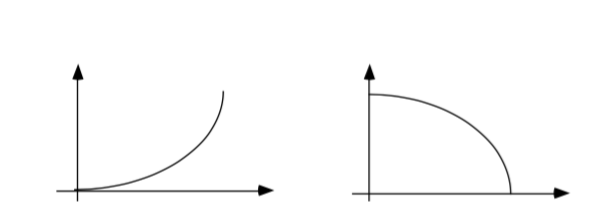
\includegraphics[scale = 0.5]{chapters/chapter04/fig04/5.png}}
\caption{Monotone linguistic quantifiers}
\label{pig:owa5}
\end{figure}
\begin{figure}[h]
\vspace{.2in}
\centering{
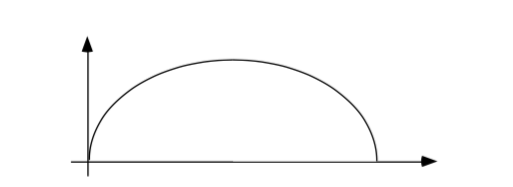
\includegraphics[scale = 0.5]{chapters/chapter04/fig04/6.png}}
\caption{Unimodal linguistic quantifier}
\label{pig:owa6}
\end{figure}

With $a_i = A_i(x)$ the overall valuation of $x$ is $F_Q(a_1,\dots,a_d)$ where $F_Q$ is an OWA operator. The weights associated with this quantified guided aggregation are obtained as follows 
\begin{equation}
\label{equa:owa5}
w_i = Q(\frac{i}{d}) - Q(\frac{i-1}{d}) , i = 1,\dots,n.
\end{equation}

From the Figure~\ref{pig:owa7} graphically shows that the operation involved in determining the OWA weights directly from the quantifier guiding the aggregation.
\begin{figure}[h]
\vspace{.2in}
\centering{
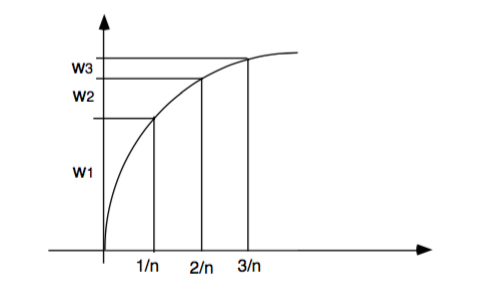
\includegraphics[scale = 0.5]{chapters/chapter04/fig04/7.png}}
\caption{Determining weights from a quantifier.}
\label{pig:owa7}
\end{figure}

Let us look at the weights generated from some basic types of quantifiers. The quantifier, for all $Q_{\ast}$ referred to the figure~\ref{pig:owa8}, is defined such that
\[Q_{\ast}(r) = \left\{
\begin{matrix}
0 & \text{for } r<1,\\
1 & \text{for } r=1.
\end{matrix}\right.\]

Using this method for generating weights
\[w_i = Q_{\ast}(\frac{i}{d})-Q_{\ast}(\frac{i-1}{d})\]
we get 
\[w_i = \left\{
\begin{matrix}
0 & \text{  for  } i<n, \\
1 & \text{  for  } i=n.
\end{matrix}
\right.\]
\begin{figure}[h]
\vspace{.2in}
\centering{
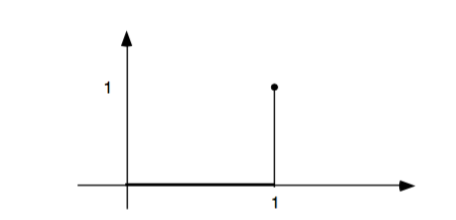
\includegraphics[scale = 0.5]{chapters/chapter04/fig04/8.png}}
\caption{The quantifier all.}
\label{pig:owa8}
\end{figure}

This is exactly what we previously denoted as $W_{\ast}$.

For the quantifier there exists (referred to the figure~\ref{pig:owa9})we have 
\[Q^{\ast}(r) = \left\{
\begin{matrix}
0 & \text{for } r=0,\\
1 & \text{for } r>0.
\end{matrix}\right.\]
\begin{figure}[h]
\vspace{.2in}
\centering{
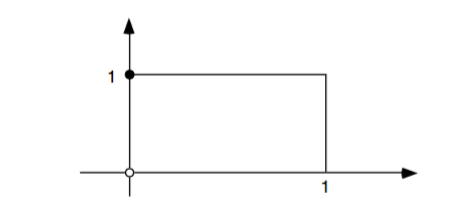
\includegraphics[scale = 0.5]{chapters/chapter04/fig04/9.png}}
\caption{The quantifier there exists.}
\label{pig:owa9}
\end{figure}

In this case we get 
\[w_1 = 1, w_i = 0, \text{  for } i\neq 1.\]
This is exactly what we denoted as $W^{\ast}$.

Consider next the quantifier referred to the figure~\ref{pig:owa10} defined by 
\[Q(r) = r.\]
\begin{figure}[h]
\vspace{.2in}
\centering{
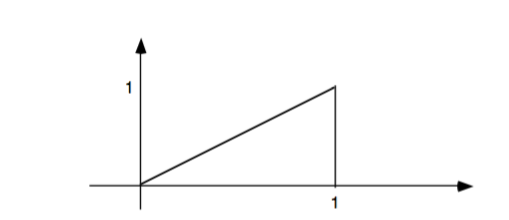
\includegraphics[scale = 0.5]{chapters/chapter04/fig04/10.png}}
\caption{The identity quantifier.}
\label{pig:owa10}
\end{figure}
This is an identity or linear type quantifier.

In this case, we get
\[w_i = Q(\frac{i}{d})-Q(\frac{i-1}{d}) = \frac{i}{d} - \frac{i-1}{d} = \frac{1}{d}.\]
This gives us the pure averaging OWA aggregation operator.

The standard degree of orness associated with a Regular Increasing Monotone (RIM) linguistic quantifier $Q$
\[\text{orness}(Q) = \int_0^1Q(r)\mathrm{d}r\]
is equal to the area under the quantifier\cite{yager1996quantifier}. This definition for the measure of orness of quantifier provides a simple useful method for obtaining this measure. 